\subsection{Backgrounds: Semileptonic channel}
\label{subsec:bkg_semilept}

Control regions for the two major backgrounds, dileptonic $\ttbar$ and $\Wjets$, are described in the following.

\subsubsection{Control region for \texorpdfstring{$\ttbar$}{ttbar}}
\label{subsubsec:bkg_semilept_ttbar}

A control region enriched in dileptonic $\ttbar$ can be obtained by requiring a $ee$, $e\mu$, and $\mu\mu$ dilepton pairs where each lepton passes ``Tight'' selection. The four-momentum of the trailing lepton is subtracted from the event to construct the $\met$ template, and is used to compute all $\met$-related variables: $M_T, M_{T2}^W, \min_{i=1,2}\Delta\phi\left(j_i,\,\met\right)$. All other selection cuts for the semileptonic channel are applied accordingly. The yields are listed in Table~\ref{tab:semilept_bkg_tt2l_yields}. The lepton subtracted $\met$ distributions in the control region for the inclusive selection is shown in Fig.~\ref{fig:incl_semilept_2l_fmet}.

\begin{table}[!ht]
\centering
\begin{tabular}{|c|rr|rr|rr|}
\hline
  Process & \multicolumn{2}{|c|}{Inclusive} & \iffalse \multicolumn{2}{|c|}{Boosted} &\fi \multicolumn{2}{|c|}{Resolved} \\
          & $e$ & $\mu$                     & \iffalse$e$ & $\mu$                   &\fi $e$ & $\mu$ \\
\hline
  \Z\To\Lep\Lep          & $  0.50 \pm 0.13$ & $  0.62 \pm 0.12$  &\iffalse $ 0.19 \pm 0.09$ & $ 0.12 \pm 0.02$  &\fi $  0.38 \pm 0.11$ & $  0.52 \pm 0.11$ \\
  Single \Top            & $ 11.80 \pm 1.46$ & $ 13.35 \pm 1.56$  &\iffalse $ 1.09 \pm 0.45$ & $ 1.64 \pm 0.55$  & \fi$ 11.25 \pm 1.43$ & $ 12.26 \pm 1.49$ \\
  \Wjets                 & $  0.03 \pm 0.03$ & $  0.03 \pm 0.03$  & \iffalse$ 0.03 \pm 0.03$ & $ 0.00 \pm 0.00$  & \fi$  0.03 \pm 0.03$ & $  0.03 \pm 0.03$ \\
  $\ttbar+V$             & $  1.86 \pm 0.16$ & $  1.86 \pm 0.03$  & \iffalse$ 0.62 \pm 0.09$ & $ 0.55 \pm 0.09$  & \fi$  1.52 \pm 0.15$ & $  1.51 \pm 0.15$ \\
  $\ttbar(\mbox{had})$   & $  0.00 \pm 0.00$ & $  0.00 \pm 0.00$  &\iffalse $ 0.00 \pm 0.00$ & $ 0.00 \pm 0.00$  & \fi$  0.00 \pm 0.00$ & $  0.00 \pm 0.00$ \\
  $\ttbar(1\Lep)$        & $  0.16 \pm 0.16$ & $  0.00 \pm 0.00$  &\iffalse $ 0.00 \pm 0.00$ & $ 0.00 \pm 0.00$  & \fi$  0.16 \pm 0.16$ & $  0.00 \pm 0.00$ \\
  $\ttbar(2\Lep)$        & $107.05 \pm 4.18$ & $112.77 \pm 4.29$  &\iffalse $13.73 \pm 1.50$ & $14.71 \pm 1.55$  &\fi $102.80 \pm 4.10$ & $108.35 \pm 4.21$ \\
\hline
  SM expected            & $121.39 \pm 4.44$ & $128.63 \pm 4.57$  &\iffalse $15.65 \pm 1.57$ & $17.01 \pm 1.65$  & \fi$116.13 \pm 4.35$ & $122.68 \pm 4.47$ \\
\hline
  $M_\chi=1\:\GeV$       & $  4.94 \pm 0.45$ & $  6.38 \pm 0.51$  &\iffalse $ 0.16 \pm 0.08$ & $ 0.53 \pm 0.15$  &\fi $  4.81 \pm 0.44$ & $  6.21 \pm 0.51$ \\
\hline
\end{tabular}
\caption{Expected yields for $5\:\ifb$ in the $\ttbar$ control region for the semileptonic channel.}
\label{tab:semilept_bkg_tt2l_yields}
\end{table}

\begin{figure}[htbp]
  \centering
  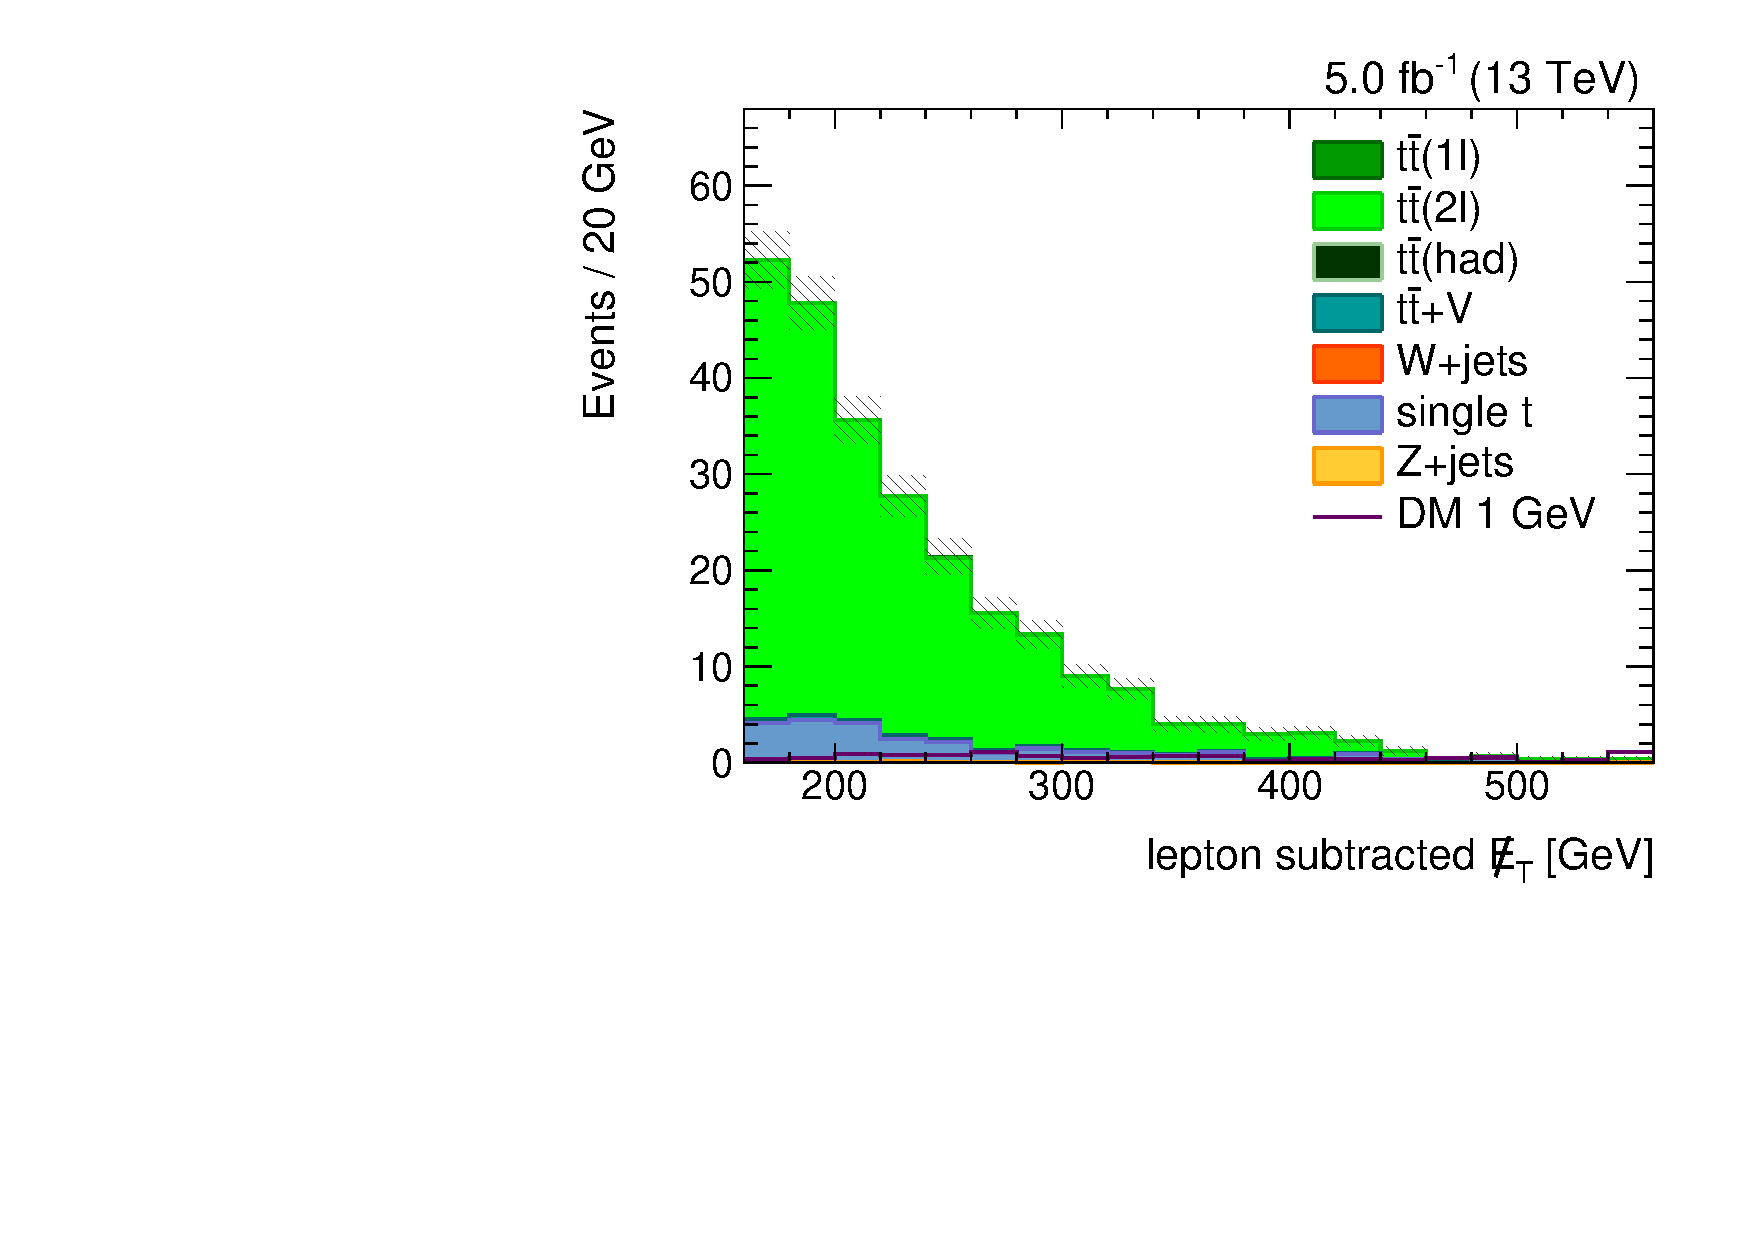
\includegraphics[width=0.48\textwidth]{figures/semilept-incl-2l-fmet_l.pdf}
  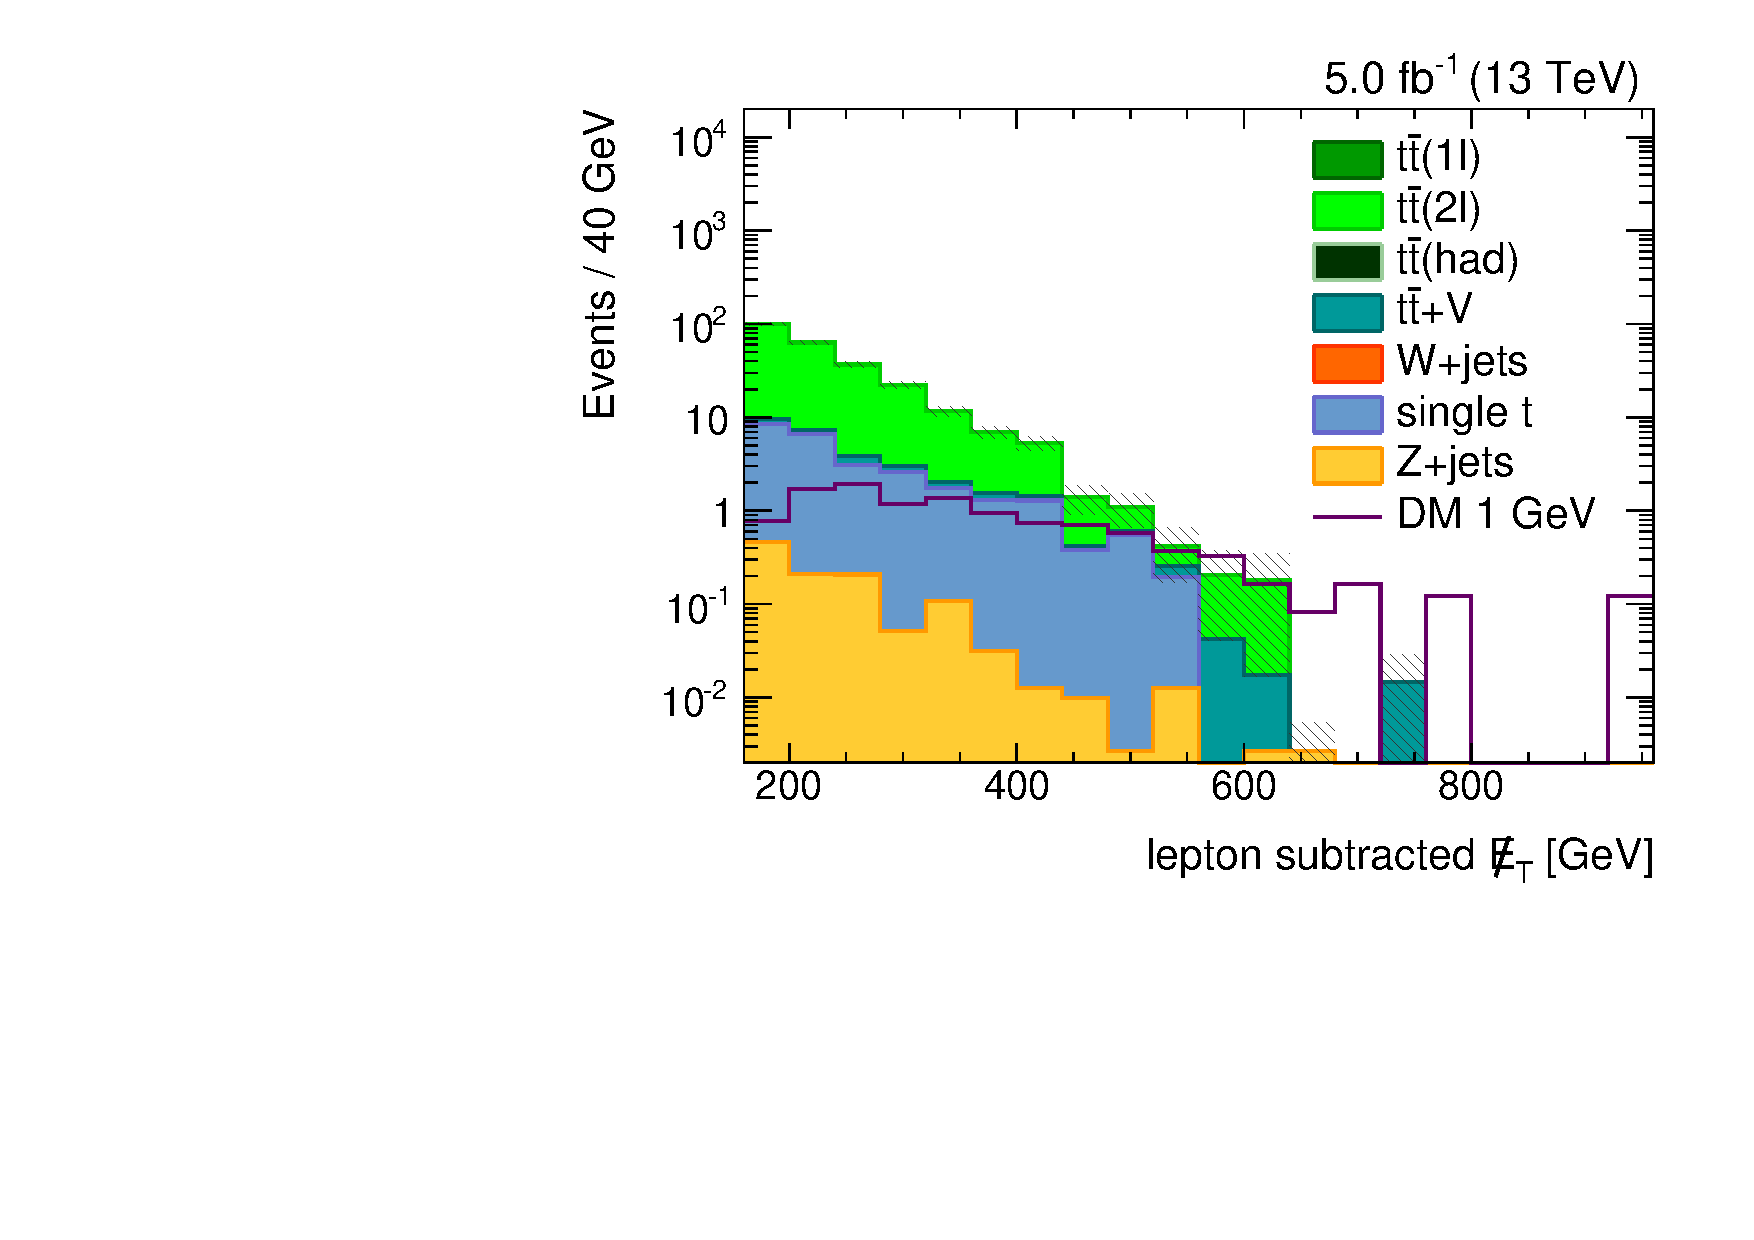
\includegraphics[width=0.48\textwidth]{figures/semilept-incl-2l-fmetlog_l.pdf}
  \caption{The $\met$ distribution in the $\ttbar$ control region for the semileptonic channel.}
  \label{fig:incl_semilept_2l_fmet}
\end{figure}

\subsubsection{Control region for \texorpdfstring{$\Wjets$}{Wjets}}
\label{subsubsec:bkg_semilept_wjets}

By requiring no $\Bot$-tagged jets in the event and keeping all other cuts the same, a sample enriched in $\Wjets$  can be obtained. \iffalse For the categories with boosted top tags, the subjet $\Bot$-tag requirements are dropped. \fi The yields are listed in Table~\ref{tab:semilept_bkg_wjets_yields}. The $\met$ distributions in the control region for the inclusive selection is shown in Fig.~\ref{fig:incl_semilept_0b_met}.

\begin{table}[!ht]
\centering
\begin{tabular}{|c|rr|rr|rr|}
\hline
  Process & \multicolumn{2}{|c|}{Inclusive} &\iffalse \multicolumn{2}{|c|}{Boosted} &\fi \multicolumn{2}{|c|}{Resolved} \\
          & $e$ & $\mu$                     & \iffalse$e$ & $\mu$                   &\fi $e$ & $\mu$ \\
\hline
  \Z\To\Lep\Lep          & $ 0.40 \pm 0.26$ & $ 0.51 \pm 0.11$  &\iffalse $ 0.12 \pm 0.03$ & $ 0.53 \pm 0.14$  & \fi$ 0.38 \pm 0.26$ & $ 0.43 \pm 0.11$ \\
  Single \Top            & $ 1.33 \pm 0.49$ & $ 1.52 \pm 0.52$  & \iffalse$ 0.55 \pm 0.32$ & $ 0.78 \pm 0.37$  &\fi $ 1.15 \pm 0.45$ & $ 1.28 \pm 0.48$ \\
  \Wjets                 & $46.58 \pm 4.47$ & $57.74 \pm 5.59$  & \iffalse$20.18 \pm 2.60$ & $24.80 \pm 2.98$  &\fi $40.75 \pm 4.33$ & $50.33 \pm 5.44$ \\
  $\ttbar+V$             & $ 0.44 \pm 0.08$ & $ 0.64 \pm 0.09$  & \iffalse$ 0.56 \pm 0.09$ & $ 0.67 \pm 0.10$  & \fi$ 0.31 \pm 0.07$ & $ 0.51 \pm 0.08$ \\
  $\ttbar(\mbox{had})$   & $ 0.00 \pm 0.00$ & $ 0.00 \pm 0.00$  & \iffalse$ 0.00 \pm 0.00$ & $ 0.00 \pm 0.00$  & \fi$ 0.00 \pm 0.00$ & $ 0.00 \pm 0.00$ \\
  $\ttbar(1\Lep)$        & $ 0.16 \pm 0.16$ & $ 0.16 \pm 0.16$  & \iffalse$ 0.33 \pm 0.23$ & $ 1.14 \pm 0.43$  & \fi$ 8.83 \pm 1.20$ & $10.79 \pm 1.33$ \\
  $\ttbar(2\Lep)$        & $ 9.97 \pm 1.28$ & $12.09 \pm 1.41$  &\iffalse $ 8.17 \pm 1.16$ & $ 9.15 \pm 1.22$  & \fi$ 0.16 \pm 0.16$ & $ 0.16 \pm 0.16$ \\
\hline
  SM expected            & $58.88 \pm 4.69$ & $72.67 \pm 5.79$  &\iffalse $29.89 \pm 2.87$ & $37.07 \pm 3.27$  & \fi$51.57 \pm 4.53$ & $63.50 \pm 5.63$ \\
\hline
  $M_\chi=1\:\GeV$       & $10.24 \pm 0.65$ & $12.01 \pm 0.70$  & \iffalse$ 6.62 \pm 0.52$ & $ 8.35 \pm 0.59$  &\fi $ 7.69 \pm 0.56$ & $ 8.43 \pm 0.59$ \\
\hline
\end{tabular}
\caption{Expected yields for $5\:\ifb$ in the $\Wjets$ control region for the semileptonic channel.}
\label{tab:semilept_bkg_wjets_yields}
\end{table}

\begin{figure}[htbp]
  \centering
  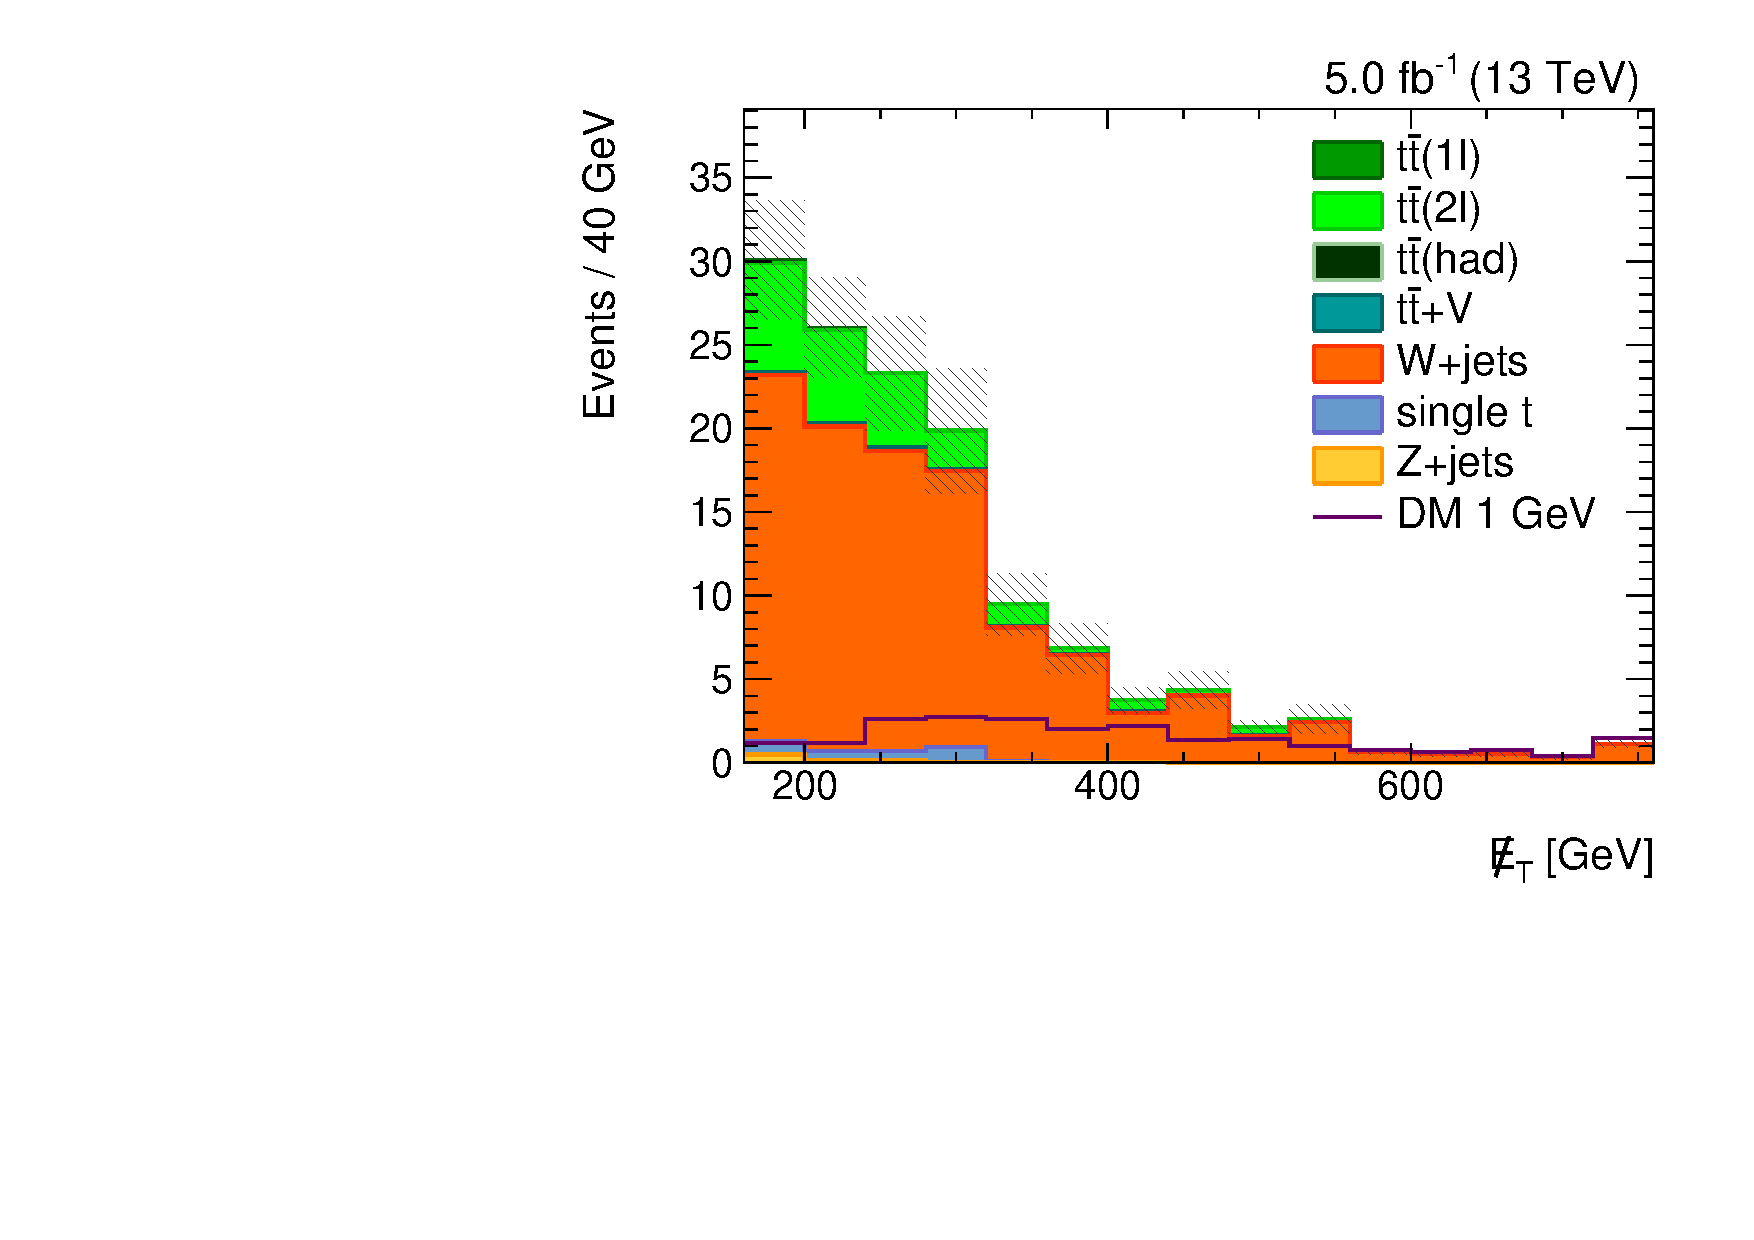
\includegraphics[width=0.48\textwidth]{figures/semilept-incl-0b-met_l.pdf}
  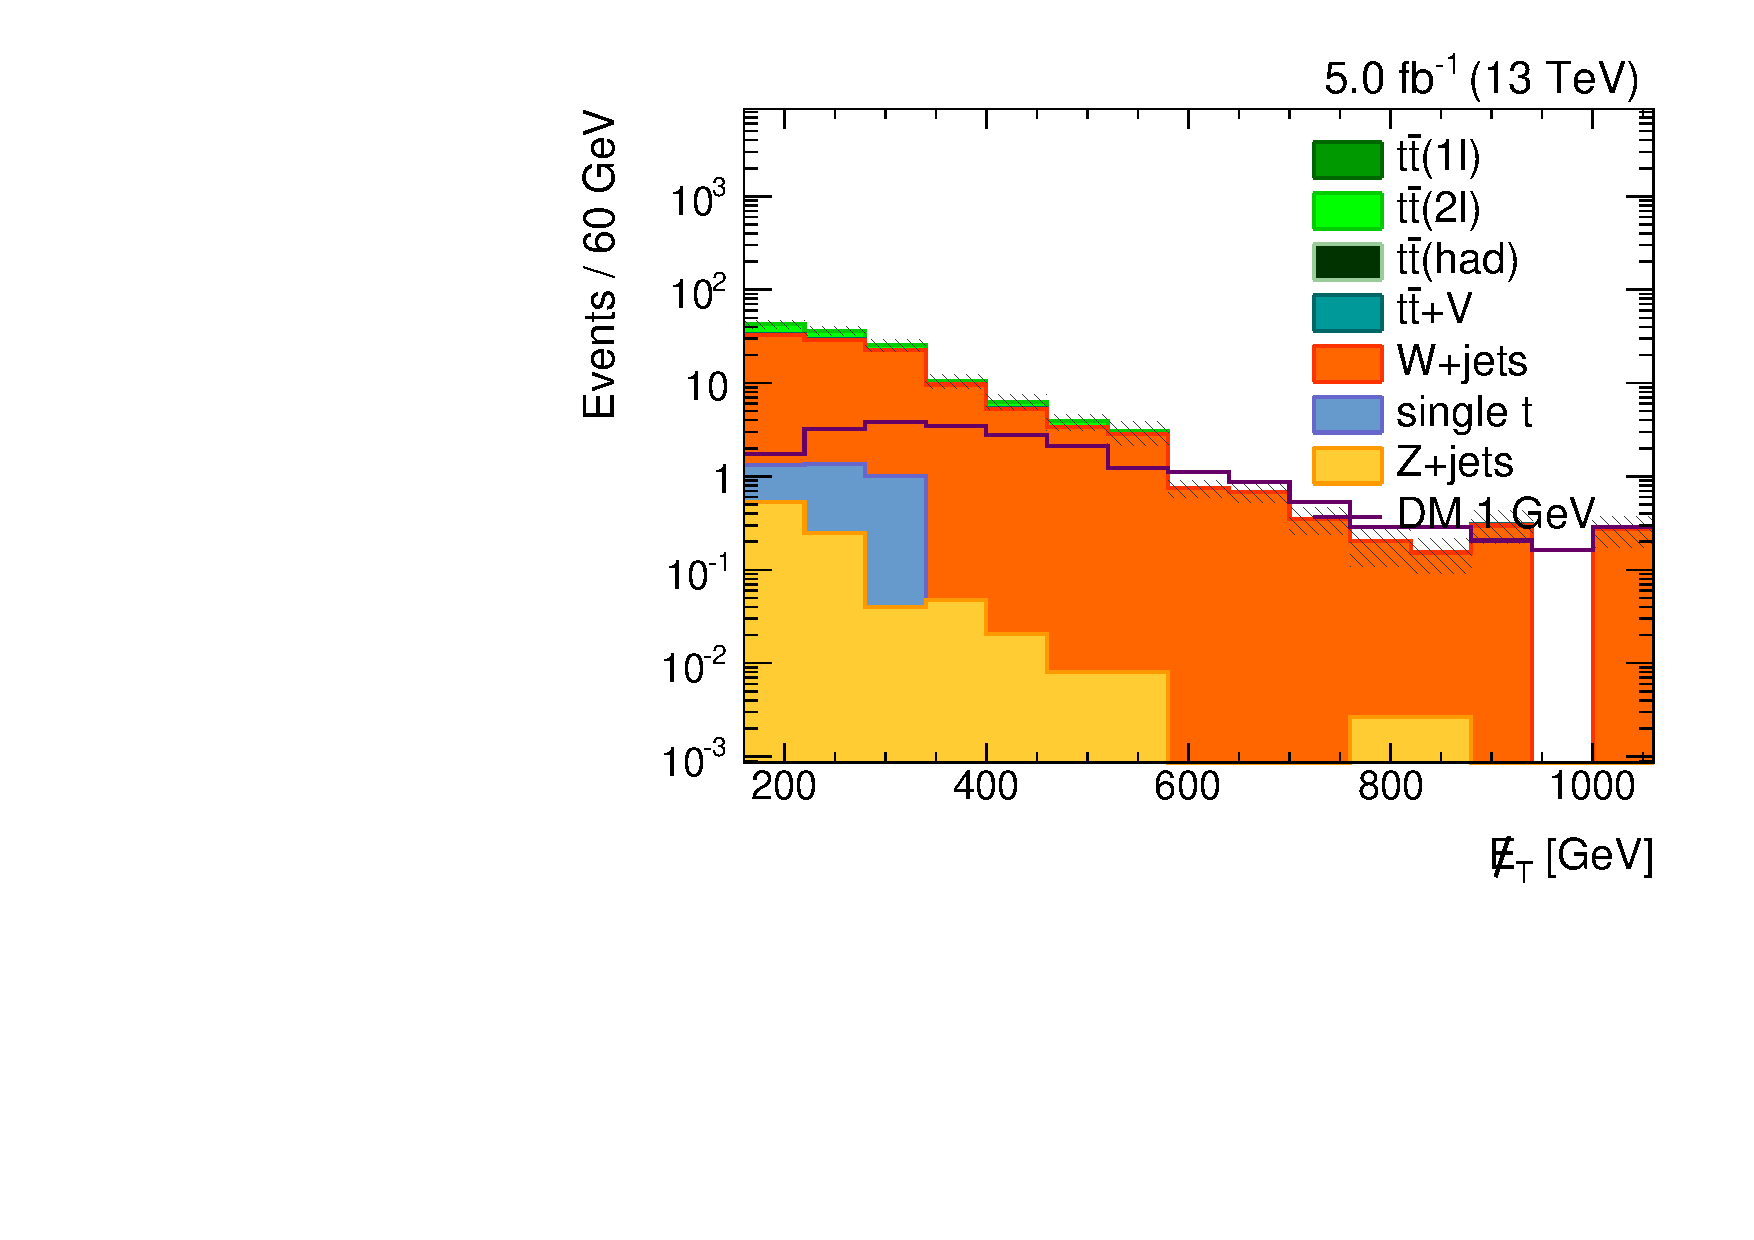
\includegraphics[width=0.48\textwidth]{figures/semilept-incl-0b-metlog_l.pdf}
  \caption{The $\met$ distribution in the $\Wjets$ control region for the semileptonic channel.}
  \label{fig:incl_semilept_0b_met}
\end{figure}
